\section{Data overview}

Figure~\ref{fig:daily} illustrates the temporal support and units of selected measurements. Daily participation and payments are available for different retained populations, while UMA delay describes completed requests and Flare concentration describes epoch-specific signing policies. These quantities are interpreted within their branch, role and observation window. Open requests remain in the lifecycle records, days without eligible retained events remain unfilled, and policy weights are kept separate from token amounts. The broader feasibility assessment in Appendix~\ref{app:daily} identifies which comparisons require additional evidence.
\begin{figure}[!htbp]
\centering
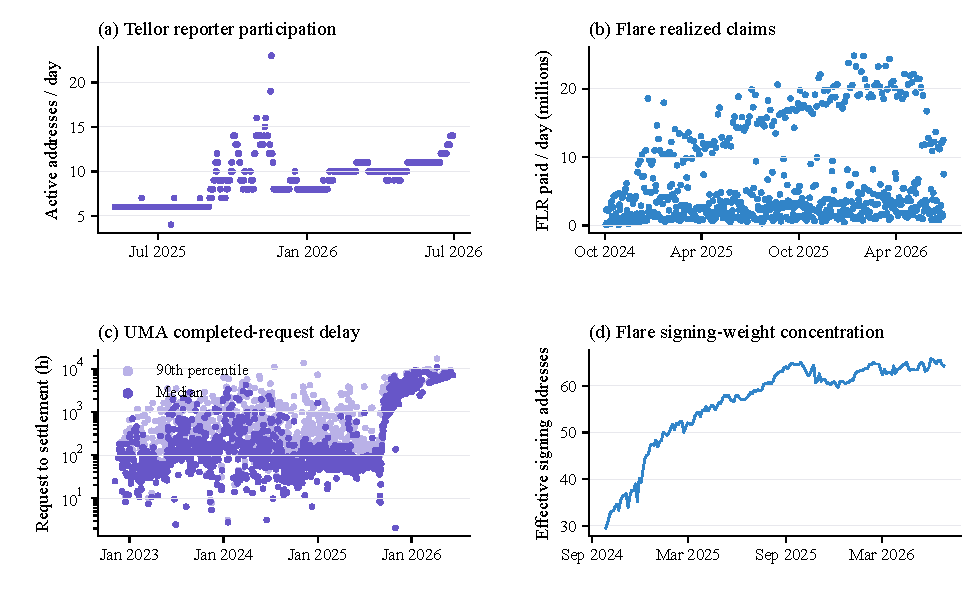
\includegraphics[width=0.99\linewidth]{figures/daily_gallery.pdf}
\caption{Selected measurements from the daily product and its epoch-level companion. (a) Distinct Tellor reporter addresses with retained reports on each observed day. (b) Flare claims in FLR, excluding fee burns. (c) Median and 90th-percentile request-to-settlement delay among flow-reconciled UMA USDC.e requests completed on that day; the vertical axis is logarithmic. (d) Effective signing-address count, $1/\sum_i w_i^2$, using normalized Flare signing-policy weights within each retained epoch. Address counts do not identify independent entities.}
\label{fig:daily}
\end{figure}
